On considère un système oscillant (solide-ressort horizontal) où la valeur de la
masse du solide est $m=\qty{125}{\gram}$ et la raideur du ressort est noté $K$.

\begin{minipage}{0.65\linewidth}
    L'équation horaire du mouvement du centre d'inertie $G$ du solide s'écrit
    $x=X_m \cos \left(\frac{2\pi}{T_0} t\right)$.

    La courbe de la Fig.~\ref{fig:2bac_svt_national_2024_normale_phys_ex3_2}
    représente l'élongation $x$ du mouvement de $G$.

    \begin{enumerate}
        \item Déterminer graphiquement les valeurs des grandeurs $X_m$ et
              $T_0$.
        \item Vérifier que $K=\qty{19.7}{\newton\per\meter}$
        \item Déterminer l'intensité de la force de rappel exercée par le
              ressort sur le solide a l'instant $t=\frac{5}{2} T_0$.
    \end{enumerate}
\end{minipage}
\hfill
\begin{minipage}{0.34\linewidth}
\begin{figure}[H]
    \centering
    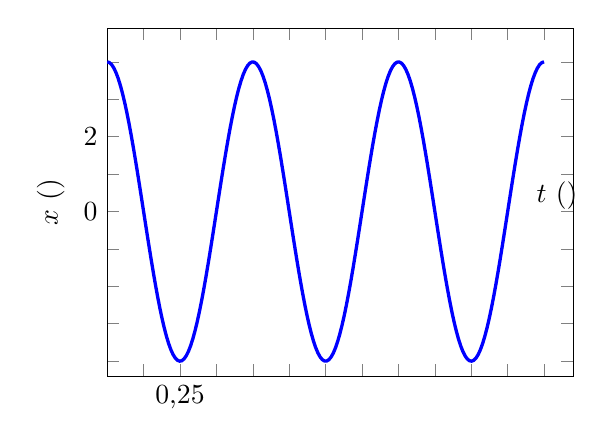
\begin{tikzpicture}
        \def\Xm{4}
        \def\T{0.5}
        \pgfmathpi\let\pi=\pgfmathresult
        \begin{axis}[
                xmin=0,xmax=3.2*\T,
                ymin=-4.4,ymax=4.9,
                width=7.5cm,height=6cm,
                trig format plots=rad,
                xtick distance=0.125, ytick distance=1,
                xticklabels={,,,{0,25}}, yticklabels={,,,,,0,,2},
                xlabel=$t~(\unit{\second})$, ylabel=$x~(\unit{\cm})$,
                every axis x label/.append style={
                	at={(1.03,0.45)},anchor=south east,
                },
                minor tick num=0,
            ]
            \addplot[domain=0:3*\T,samples=200,very thick,blue]
                {\Xm*cos(2*pi/\T*x)};
        \end{axis}
    \end{tikzpicture}
    \caption{}
    \label{fig:2bac_svt_national_2024_normale_phys_ex3_2}
\end{figure}
\end{minipage}

